%%
% This is an Overleaf template for presentations
% using the TUM Corporate Desing https://www.tum.de/cd
%
% For further details on how to use the template, take a look at our
% GitLab repository and browse through our test documents
% https://gitlab.lrz.de/latex4ei/tum-templates.
%
% The tumbeamer class is based on the beamer class.
% If you need further customization please consult the beamer class guide
% https://ctan.org/pkg/beamer.
% Additional class options are passed down to the base class.
%
% If you encounter any bugs or undesired behaviour, please raise an issue
% in our GitLab repository
% https://gitlab.lrz.de/latex4ei/tum-templates/issues
% and provide a description and minimal working example of your problem.
%%


\documentclass[
  german,            % define the document language (english, german)
  aspectratio=169,    % define the aspect ratio (169, 43)
  % handout=2on1,       % create handout with multiple slides (2on1, 4on1)
  % partpage=false,     % insert page at beginning of parts (true, false)
  % sectionpage=true,   % insert page at beginning of sections (true, false)
]{tumbeamer}


% load additional packages
\usepackage{booktabs}
\usepackage[siunitx, european]{circuitikz}


% presentation metadata
\title{Development and Enhancement\\of a Lightweight Robotic Arm}
\subtitle{with Torque Control Exploration}
\author{Tim Heger}

\institute{\theChairName\\\theDepartmentName\\\theUniversityName}
\date[03/12/2025]{3. Dezember 2025}

\footline{\insertauthor~|~\insertshorttitle~|~\insertshortdate}


% macro to configure the style of the presentation
\TUMbeamersetup{
  title page = TUM tower,         % style of the title page
  part page = TUM toc,            % style of part pages
  section page = TUM toc,         % style of section pages
  content page = TUM more space,  % style of normal content pages
  tower scale = 1.0,              % scaling factor of TUM tower (if used)
  headline = TUM threeliner,      % which variation of headline to use
  footline = TUM default,         % which variation of footline to use
  % configure on which pages headlines and footlines should be printed
  headline on = {title page},
  footline on = {every page, title page=false},
}

% available frame styles for title page, part page, and section page:
% TUM default, TUM tower, TUM centered,
% TUM blue default, TUM blue tower, TUM blue centered,
% TUM shaded default, TUM shaded tower, TUM shaded centered,
% TUM flags
%
% additional frame styles for part page and section page:
% TUM toc
%
% available frame styles for content pages:
% TUM default, TUM more space
%
% available headline options:
% TUM empty, TUM oneliner, TUM twoliner, TUM threeliner, TUM logothreeliner
%
% available footline options:
% TUM empty, TUM default, TUM infoline


\begin{document}

\maketitle

\section{Einführung}
\begin{frame}{Einführung}{}
  \centering
    \vfill
    \begin{minipage}{0.45\textwidth}
      \centering
      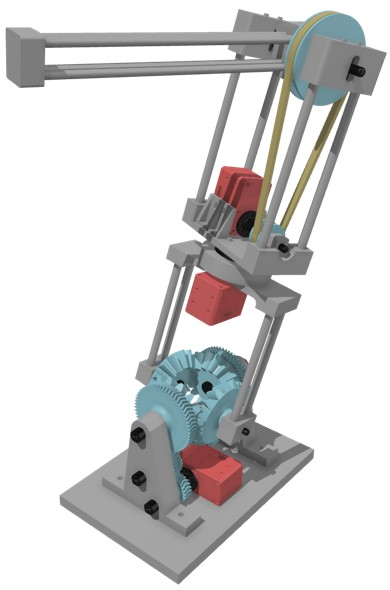
\includegraphics[height=0.6\textheight]{../900_Report/images/prev_robotic_arm_clean.jpg}
      \captionof{figure}{Vorherige Version des Roboterarms von Samuel Zeitler}
    \end{minipage}
    \hfill
    \begin{minipage}{0.45\textwidth}
      \centering
      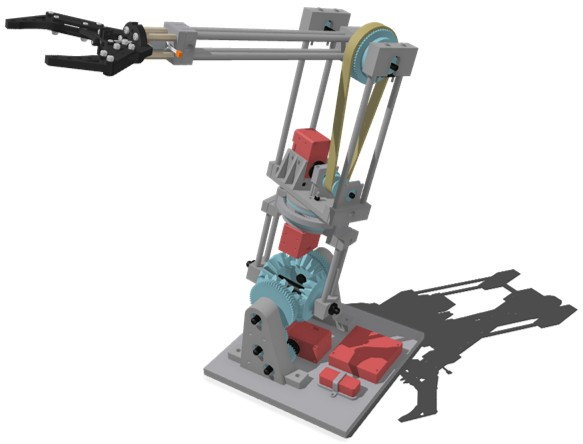
\includegraphics[height=0.6\textheight]{../900_Report/images/robot_arm_final_v2.jpg}
      \captionof{figure}{Verbesserter Roboterarm als Ergebnis dieser Arbeit}
    \end{minipage}
    \vfill
\end{frame}
  
\section{Hardware Verbesserungen}
\begin{frame}{Hardware Verbesserungen}{Mechanische Verstärkungen}
  \centering
    \vfill
    \begin{minipage}{0.25\textwidth}
      \begin{itemize}
        \item Achsen aus Aluminium gedreht
        \item Kugellager hinzugefügt
        \item Basis und Seitenstreben aus Aluminium gefräst
      \end{itemize}
    \end{minipage}
    \hfill
    \begin{minipage}{0.65\textwidth}
      \centering
      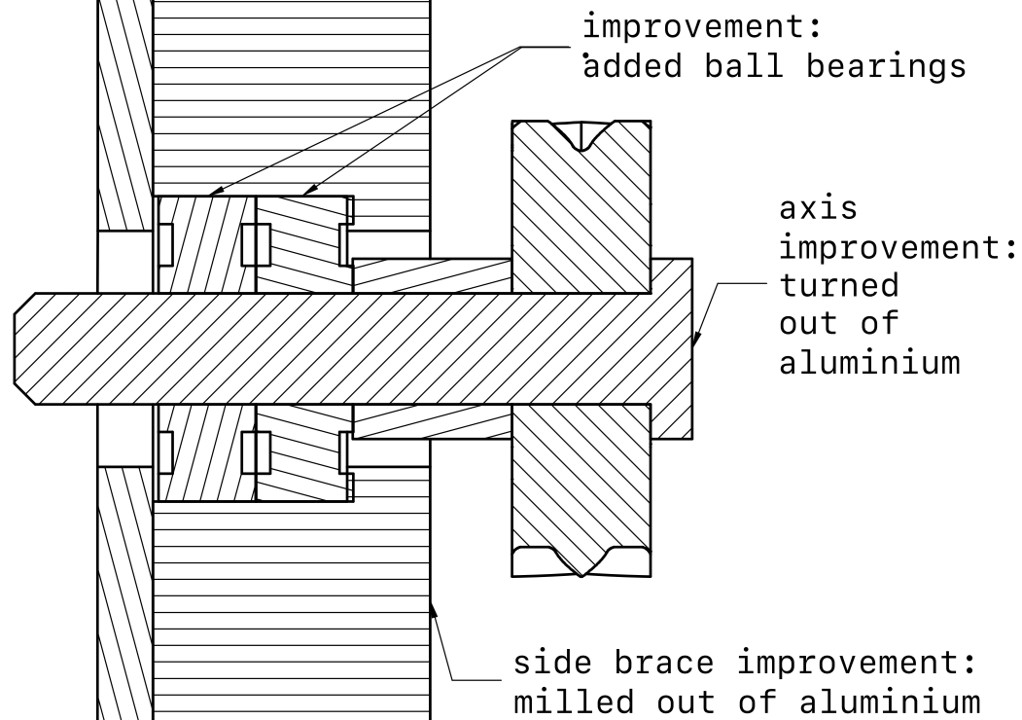
\includegraphics[height=0.6\textheight]{../900_Report/images/shoulderjoint_improvements.jpg}
      \captionof{figure}{Beispielhafte Ansicht der Hardwareverbesserungen am Schultergelenk}
    \end{minipage}
    \vfill
\end{frame}

\begin{frame}{Hardware Verbesserungen}{Planetengetriebe}
  \centering
    \vfill
    \begin{minipage}{0.5\textwidth}
      \centering
      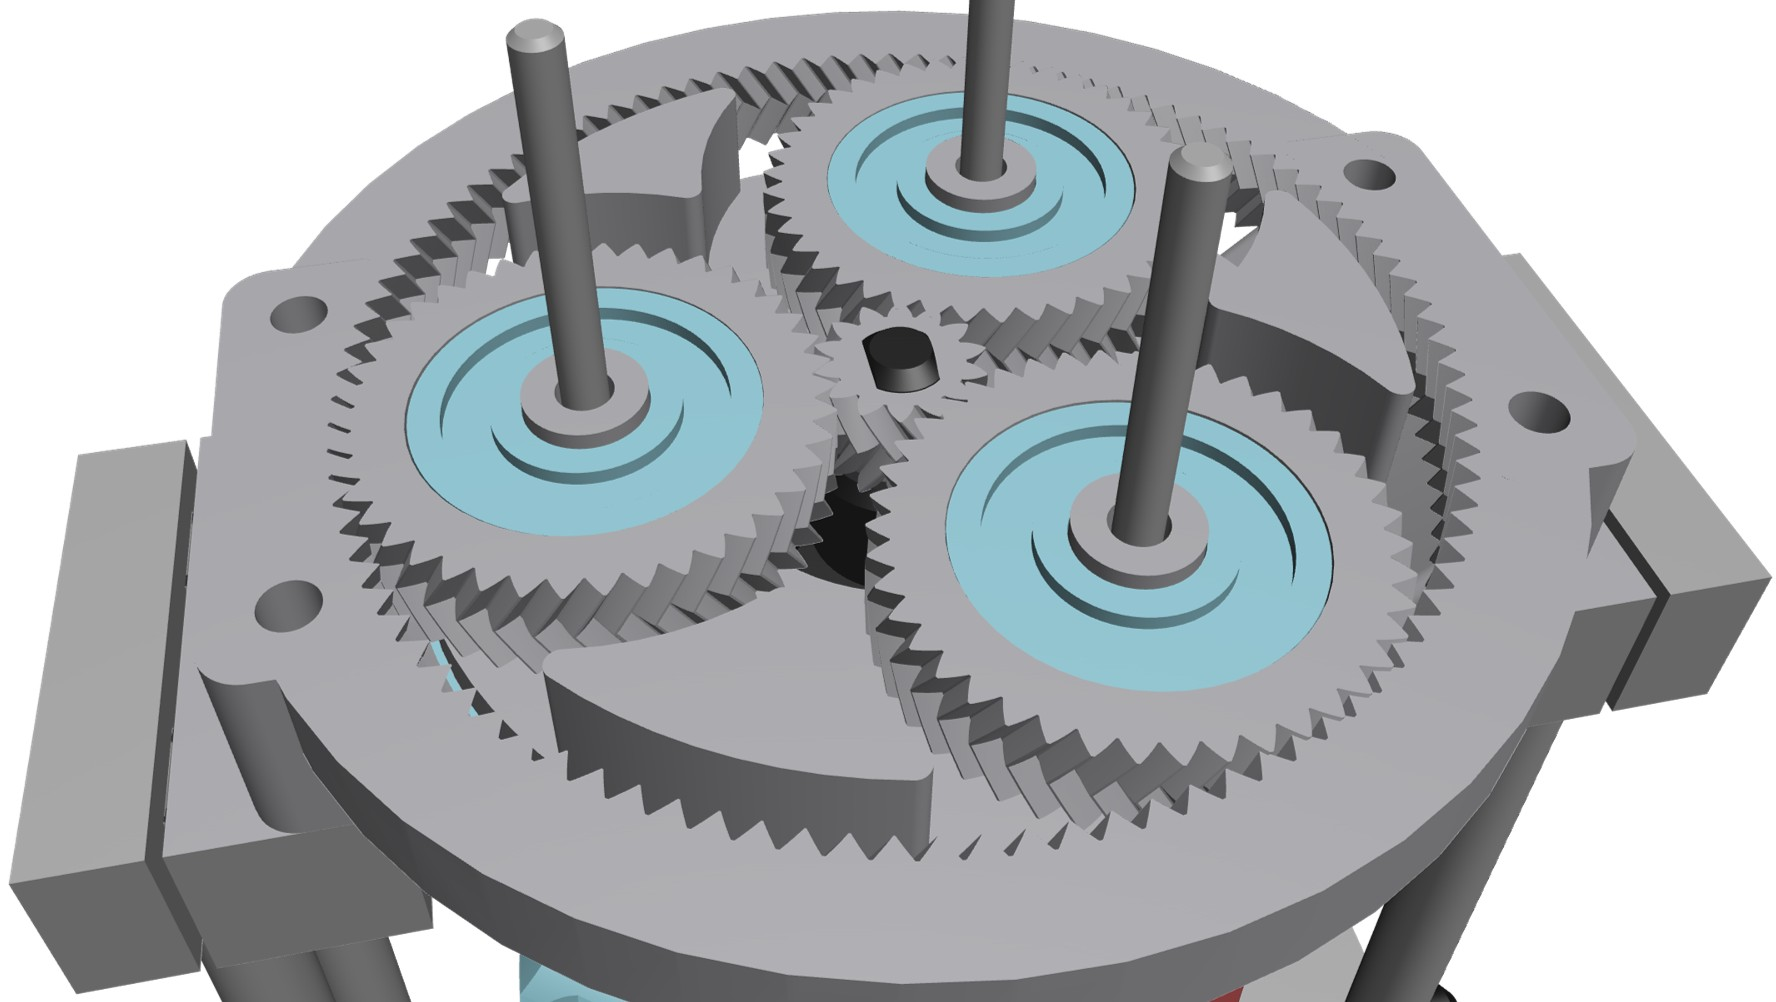
\includegraphics[width=\textwidth]{../900_Report/images/planetary_gearbox_section.jpg}
      \captionof{figure}{Ansicht der Zahnräder, entworfen mit einer OpenSCAD-Vorlage}
    \end{minipage}
    \hfill
    \begin{minipage}{0.4\textwidth}
      \centering
      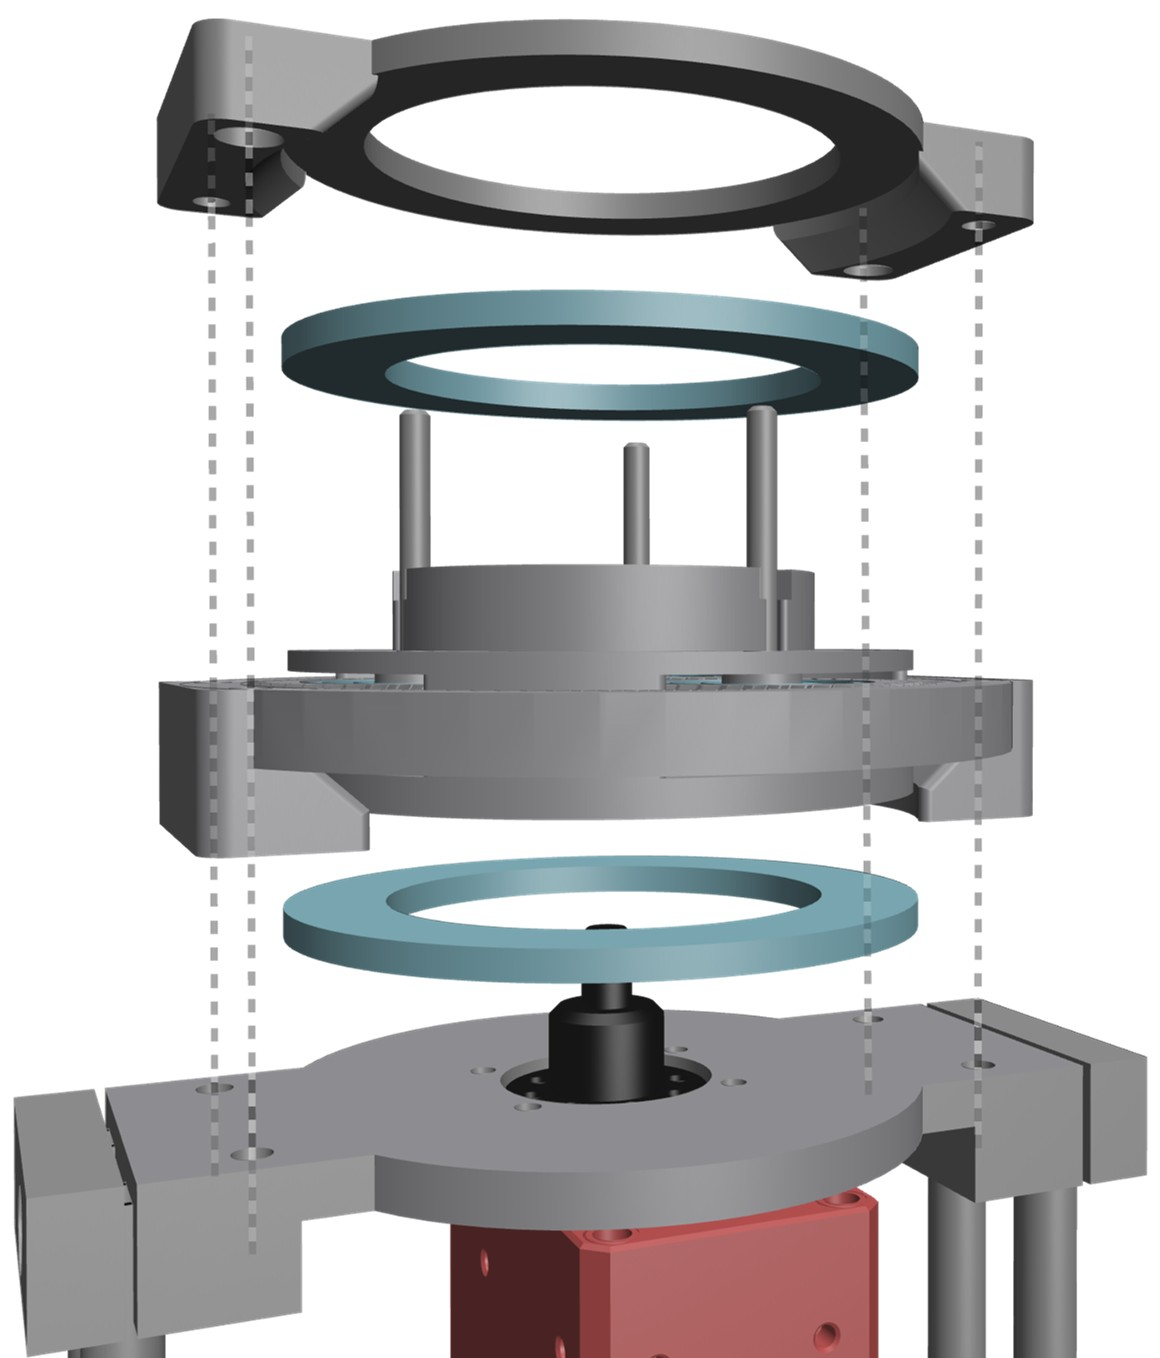
\includegraphics[height=0.6\textheight]{../900_Report/images/planetary_gearbox_explosion.jpg}
      \captionof{figure}{Darstellung der Konstruktion des Planetengetriebes}
    \end{minipage}
    \vfill  
\end{frame}

\begin{frame}{Hardware Verbesserungen}{Endeffektor}
  \centering
    \vfill
    \begin{minipage}{0.4\textwidth}
      \centering
      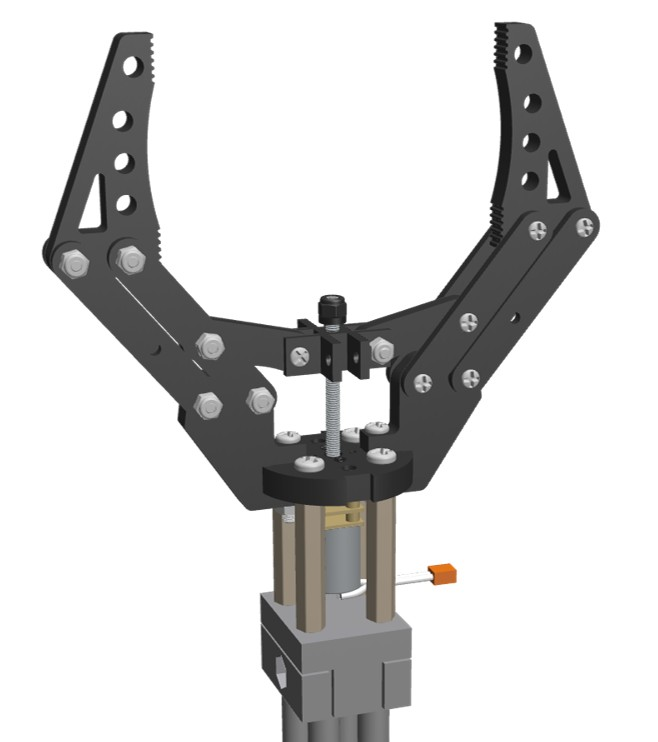
\includegraphics[height=0.6\textheight]{../900_Report/images/gripper.jpg}
      \captionof{figure}{Greifhand mit zwei Fingern als Endeffektor}
    \end{minipage}
    \hfill
    \begin{minipage}{0.5\textwidth}
      \centering
      \begin{circuitikz}
          \draw
          (0,2) node[left]{5V} to [short, o-] (0.5,2)
          (0,0.5) node[left]{GND} to [short, o-] (0.5,0.5)
          (1,2) node[spdt] {}
          (1,0.5) node[spdt] {}
          (1.5,1.685) to [short, -] (3,1.685) to[short, -o] (3,0.815)
          (1.5,0.815) to [short, -] (5,0.815)
          (5,0.815) to[Telmech=M] (5,2.315)
          (1.5,2.315) to [short, -] (5,2.315)
          (1.5,0.185) to [short, -] (3.5,0.185) to[short, -o] (3.5,2.315)
          ;
          \draw [dashed] (1,2.1) to [short] (1,0.6);
      \end{circuitikz}
      \captionof{figure}{Shaltbild des Anschlusses der Greifhand}
    \end{minipage}
    \vfill
\end{frame}

\section{Drehmomentmessung}
\begin{frame}{Drehmomentmessung}{Expreimentaufbau}
  \centering
  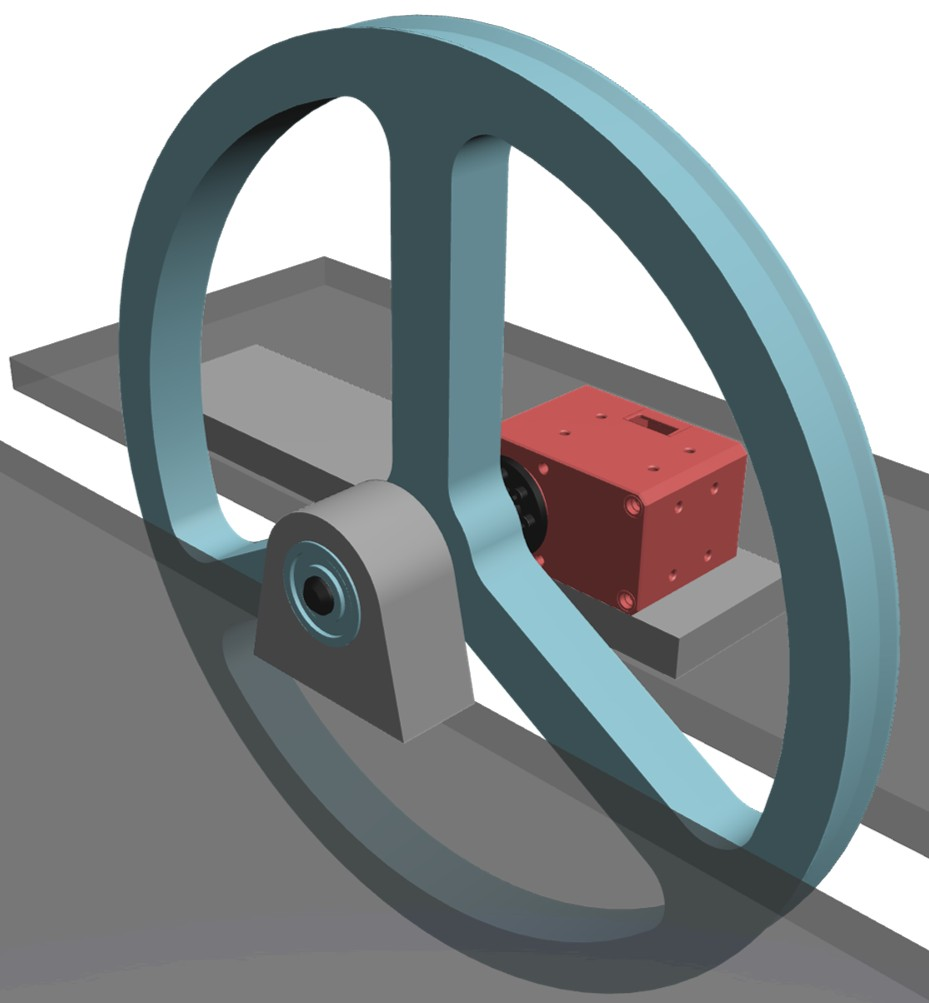
\includegraphics[height=0.6\textheight]{../900_Report/images/torque_experiment_setup.jpg}
  \captionof{figure}{Experimentaufbau zur Drehmomentmessung der Motoren}
  \vfill
\end{frame}

\begin{frame}{Drehmomentmessung}{Einteilung in drei Betriebsarten}
  \centering
  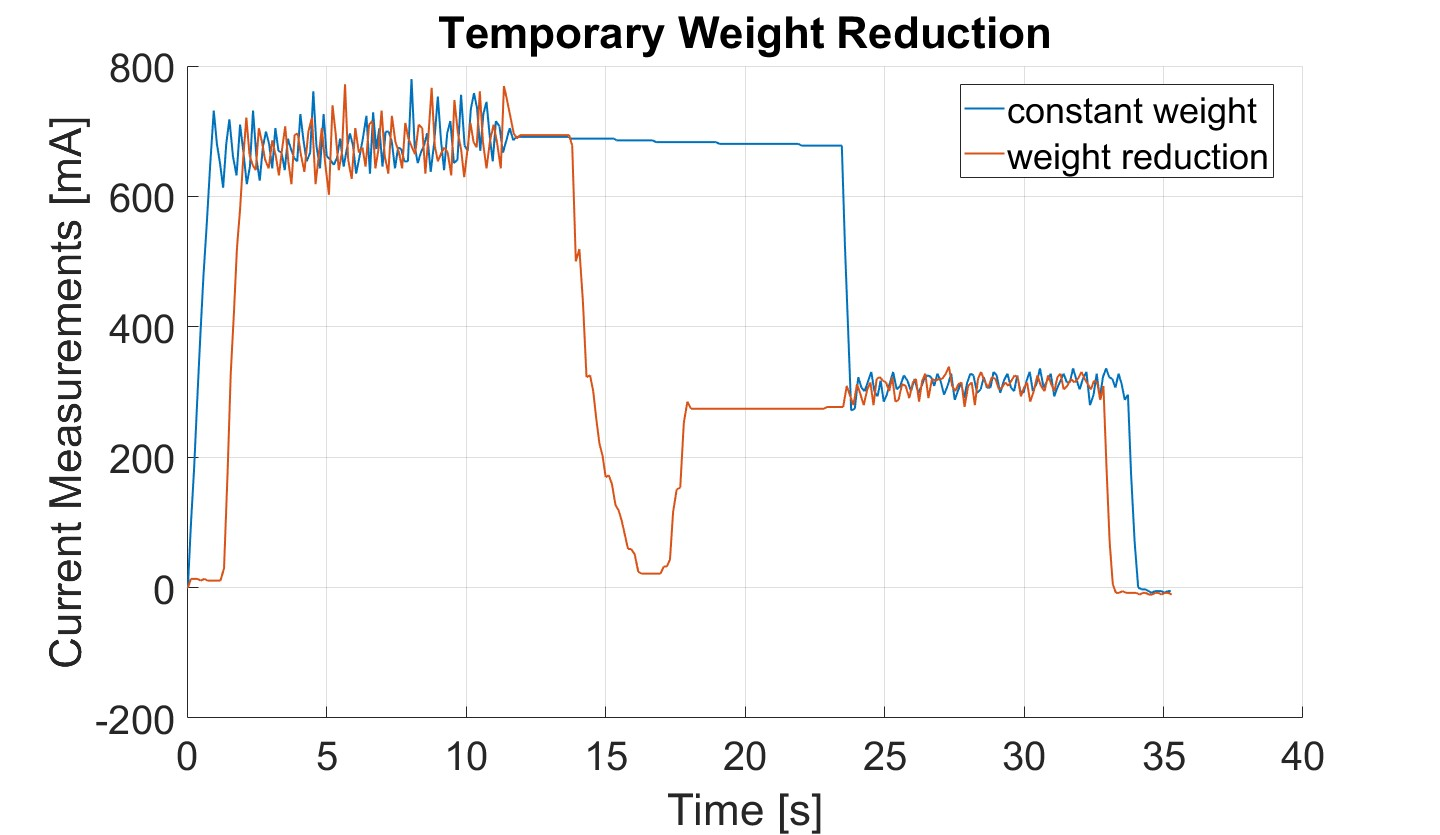
\includegraphics[height=0.6\textheight]{../900_Report/images/matlab/ex2.jpg}
  \captionof{figure}{Experiment zur Feststellung der drei Betriebsarten: Entgegenwirkender Moment, Stillstand, und mitwirkender Moment}
  \vfill  
\end{frame}

\begin{frame}{Drehmomentmessung}{Ergebnisse}
  \centering
  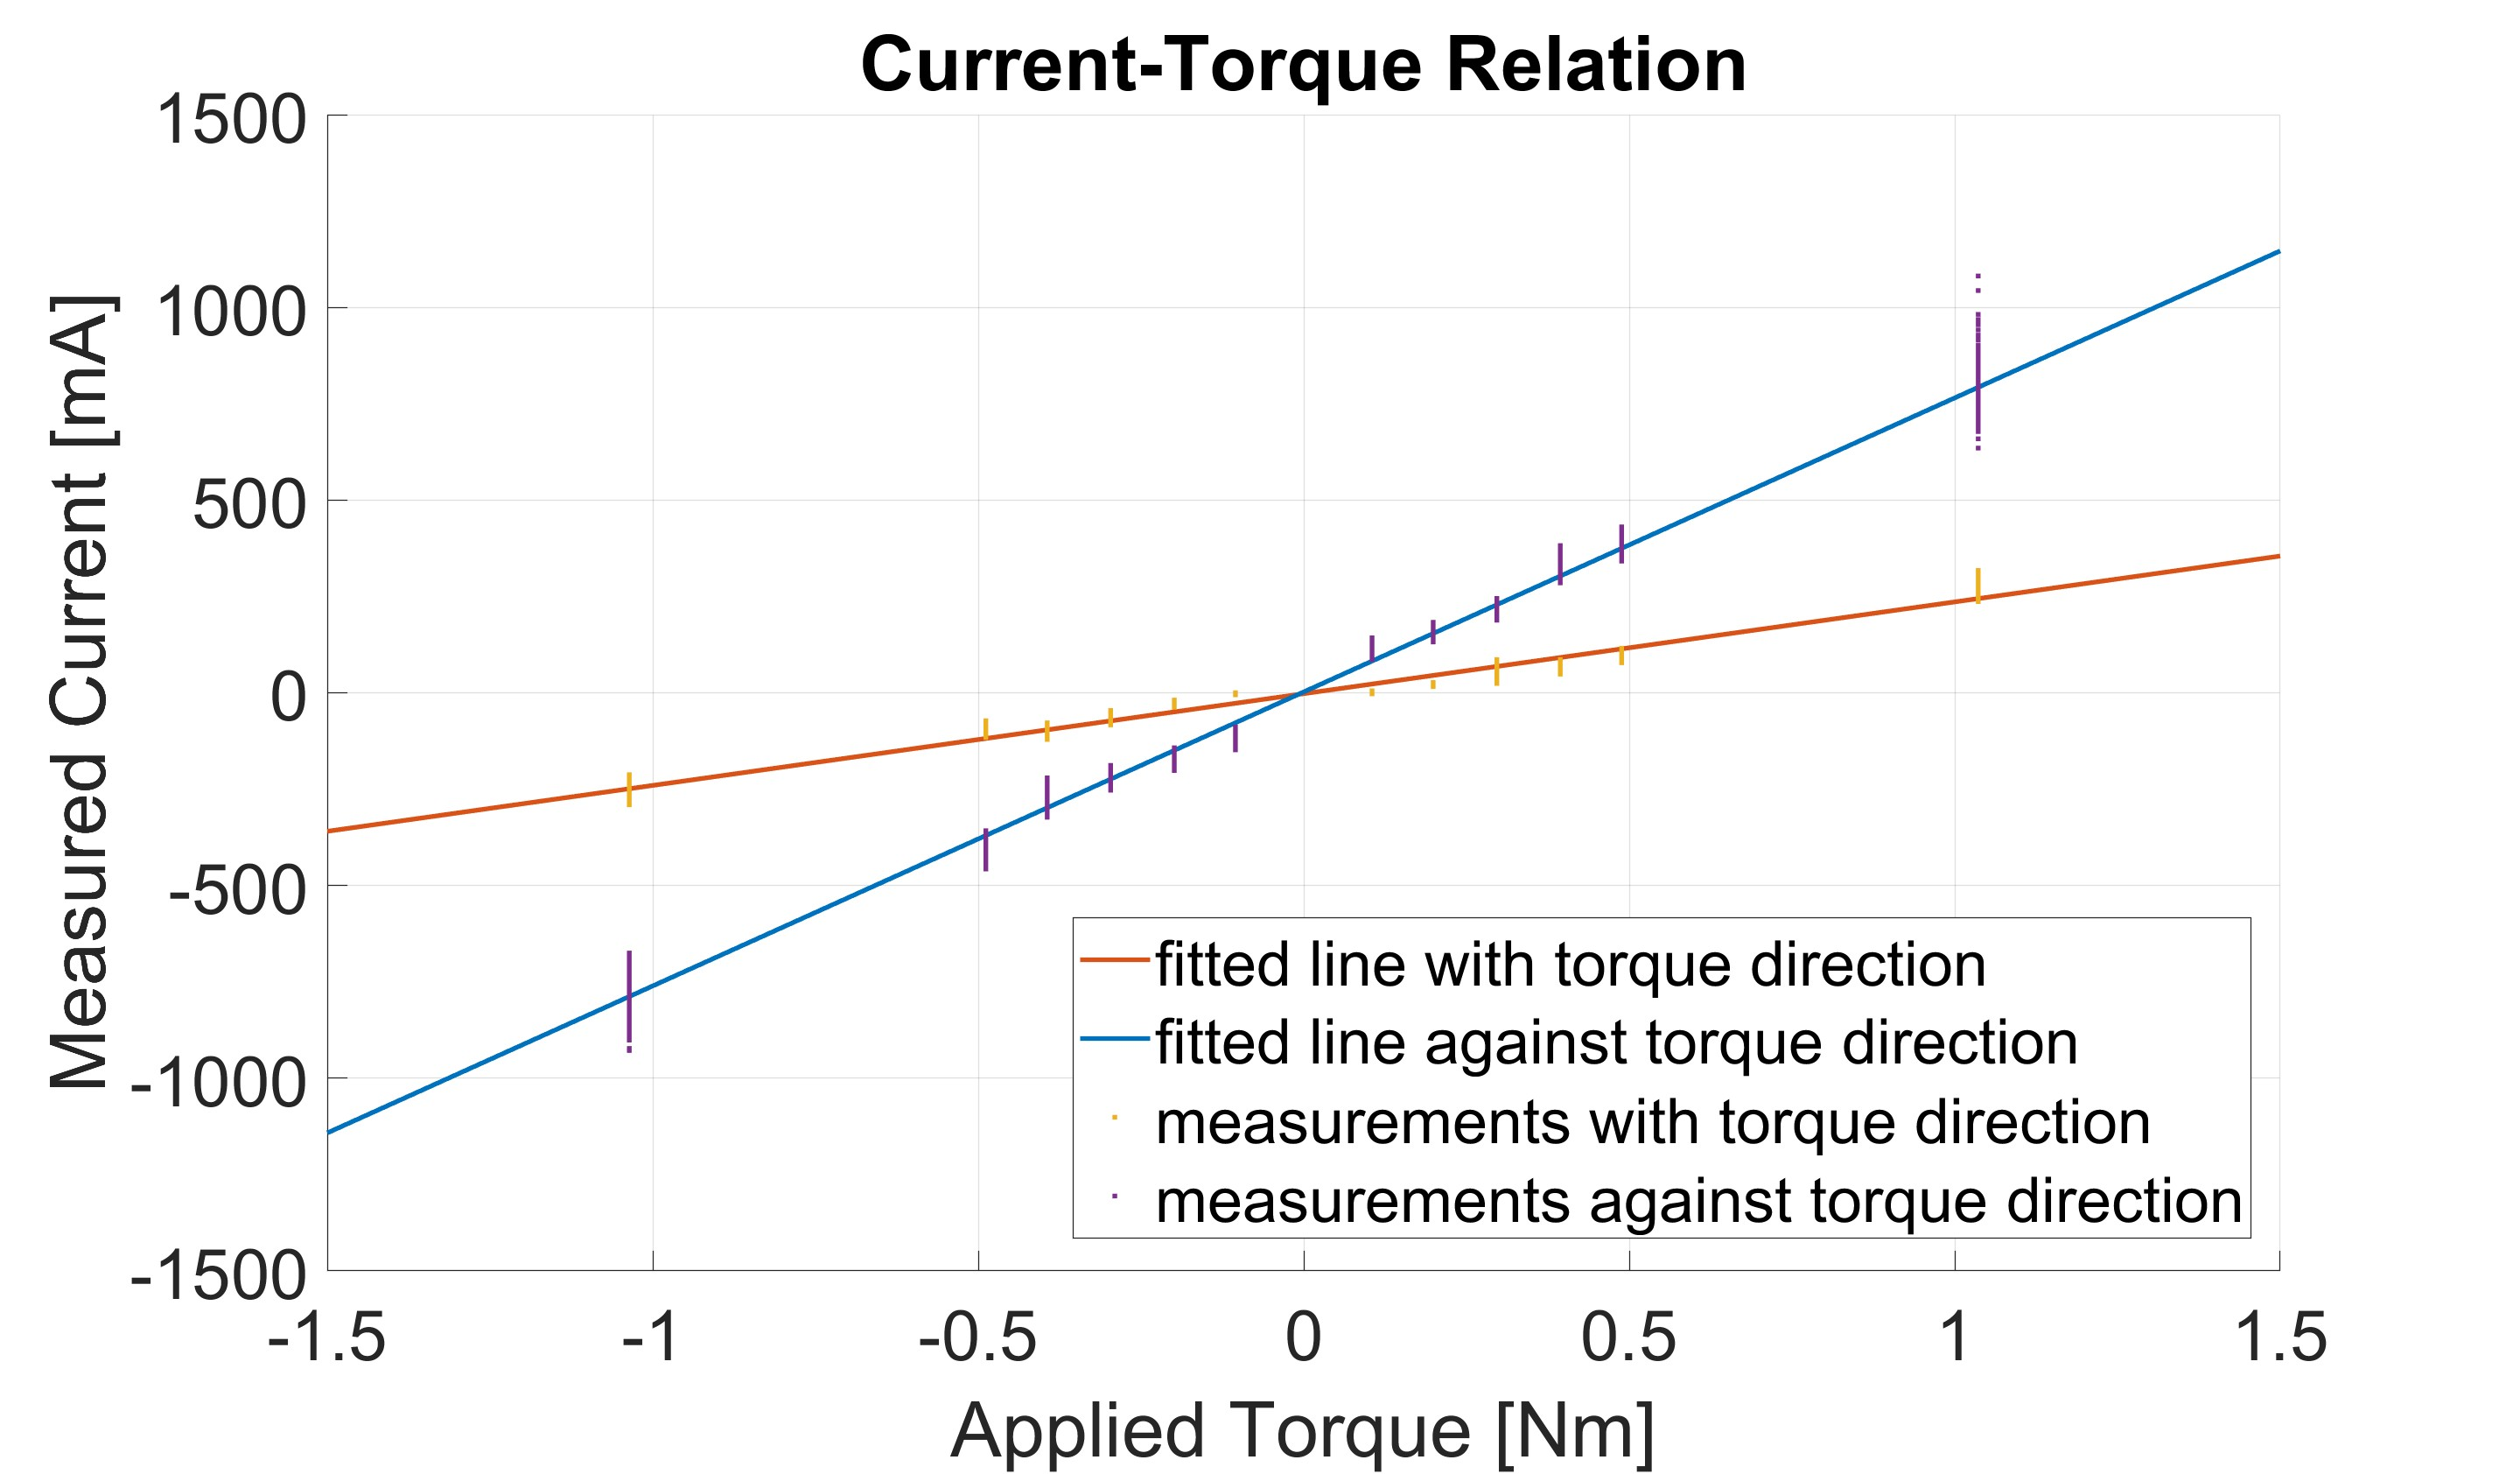
\includegraphics[height=0.6\textheight]{../900_Report/images/matlab/determine_constants_all_weights.jpg}
  \captionof{figure}{Ergebnisse der Drehmomentmessung: zwei Kennlinien für die zwei dynamischen Betriebsarten}
  \vfill
\end{frame}

\begin{frame}{Drehmomentmessung}{Implementierung einer Kräftemessung}
  \centering
  \begin{equation}
    F = (J^T)^+\,\tau
  \end{equation}
  \begin{tabular}{r@{: }l}
    Gesucht & Kraftvektor $F$ \\
    Gegeben & Jacobi-Matrix $J$ \\
    Gemessen & Drehmomentvektor der Gelenke $\tau$
  \end{tabular}
  \vfill
  \textit{Demonstration}
\end{frame}

\section{Drehmomentbasierte Regelung}
\begin{frame}{Drehmomentbasierte Regelung}{PD-Regler im Gelenkraum}
  \centering
  \begin{equation}
    \tau_{target} = - K_p \ \Delta q - K_d \ \dot{q}_{current}
  \end{equation}
  \begin{tabular}{r@{: }l}
    Gesucht & Drehmomentvektor der Gelenke $\tau_{target}$ \\
    Gegeben & Proportional- und Differentialverstärkung $K_p$ und $K_d$ \\
    Gemessen & Gelenkpositionsfehler $\Delta q$ und Gelenkgeschwindigkeitsvektor $\dot{q}_{current}$
  \end{tabular}
  \vfill
  \textit{Demonstration}
\end{frame}

\begin{frame}{Drehmomentbasierte Regelung}{PD-Regler im Kartesischen Raum}
  \centering
  \begin{align}
    F_{target} &= - K_p \ \Delta x - K_d \ \underbrace{\frac{x_{current} - x_{previous}}{\Delta t}}_{\dot{x}} \\
      \tau_{target} &= \underbrace{J^T \ F_{target}}_{\tau_{task}} \ + \ \underbrace{k_{null} \ N \ \frac{\partial H}{\partial q}}_{\tau_{null}}
  \end{align}
  \begin{tabular}{r@{: }l}
    Gesucht & Drehmomentvektor der Gelenke $\tau_{target}$ \\
    Gegeben & $K_p$ und $K_d$, Jacobi-Matrix $J$, Nullraumverstärkung $k_{null}$ \\
    Errechnet & Nullraumprojektion $N$ und Kostenfunktion $\frac{\partial H}{\partial q}$ \\
    Gemessen & TCP-Positionen $\Delta x$, $x_{current}$ und $x_{previous}$, zeitintervall $\Delta t$
  \end{tabular}
  \vfill
\end{frame}

\begin{frame}{Drehmomentbasierte Regelung}{Krafterzeugung}
  \centering
  \begin{align}
    F_{target} &= F_{pd} + F_{des} \\
    F_{pd} &= - K_p \ \Delta x_{line} - K_d \ \Delta \dot{x}_{line}
  \end{align}
  \begin{tabular}{r@{: }l}
    Gesucht & TCP-Kräfte $F_{target}$ \\
    Gegeben & $K_p$ und $K_d$, zu erzeugende Kraft $F_{des}$ \\
    Errechnet & Distanz zur durch $F_{target}$ aufgespannten Linie $\Delta x_{line}$ und $\Delta \dot{x}_{line}$ \\
    Gemessen & TCP-Positionen zur Berechnung von $\Delta x_{line}$ und $\Delta \dot{x}_{line}$
  \end{tabular}
  \vfill
  \textit{Demonstration}
\end{frame}

\begin{frame}{Vielen Dank für Ihre Aufmerksamkeit!}
  \centering
  \vfill
  \Large{Haben Sie noch Fragen?\\
  Oder Anregungen für zukünftige Arbeiten?}
  \vfill
\end{frame}

\begin{frame}{Anhang}{Berechnung der Nullraumprojektion und Kostenfunktion}
  \centering
  \begin{equation}
    N = I - J^T \left( J \, J^T + \lambda_{damp}^2 \, I \right)^{-1} J
  \end{equation}
  \begin{tabular}{r@{: }l}
    Gesucht & Nullraumprojektion $N$ \\
    Gegeben & Dämpfungsfaktor $\lambda_{damp}$, Einheitsmatrix $I$, Jacobi-Matrix $J$
  \end{tabular}
  \begin{align}
    \frac{\partial H}{\partial q} &= \underbrace{\operatorname{diag}\left(\frac{1}{q_{max}^2}\right)}_{\text{Gewichtsmatrix } W} \ (q - q_{des})
  \end{align}
  \begin{tabular}{r@{: }l}
    Gesucht & Ableitung der Kostenfunktion $\frac{\partial H}{\partial q}$ \\
    Gegeben & gewünschte Gelenkposition $q_{des}$, maximale Gelenkposition $q_{max}$ \\
    Gemessen & aktuelle Gelenkposition $q$
  \end{tabular}
\end{frame}

\begin{frame}{Anhang}{Berechnung der Distanz zur Kraftlinie}
  \centering
  \begin{align}
    \Delta x_{line} &= \Delta x - \frac{(\Delta x \cdot F_{des})}{\operatorname{norm}(F_{des})^2} \cdot F_{des} \\
    \Delta \dot{x}_{line} &= \frac{\Delta x_{line, curr} - \Delta x_{line, prev}}{\Delta t}
  \end{align}
  \begin{tabular}{r@{: }l}
    Gesucht & Distanz zur Kraftlinie $\Delta x_{line}$ und $\Delta \dot{x}_{line}$ \\
    Gegeben & gewünschte Kraft $F_{des}$ \\
    Gemessen & TCP-Positionen zur Berechnung von $\Delta x$, Zeitintervall $\Delta t$
  \end{tabular}
\end{frame}
% \section{First Section}
% \begin{frame}{Frame Title}{Subtitle}
%   \begin{itemize}
%     \item This is the first frame.
%     \item It contains some bullet points.
%   \end{itemize}
% \end{frame}

% \begin{frame}{Anoter frame of section one}
%   \centering
%   \vfill
%   \begin{tabular}{llcr}
%     \toprule
%     first & second & third & fourth \\
%     \midrule
%     1     & 2      & 3     & 4      \\
%     10    & 20     & 30    & 40     \\
%     100   & 200    & 300   & 400    \\
%     \bottomrule
%   \end{tabular}
%   \vfill
% \end{frame}

% \section{Second Section}
% \begin{frame}{Frame of section two}
%   \begin{enumerate}
%     \item one
%     \item two
%     \item three
%     \item four
%   \end{enumerate}
% \end{frame}

\end{document}
